\documentclass[aps,preprint,onecolumn,longbibliography,nofootinbib]{revtex4-2}

% ================== Packages ==================
\usepackage[utf8]{inputenc}
\usepackage[T1]{fontenc}
\usepackage{amsmath,amssymb,amsfonts}
\usepackage{bm}
\usepackage{graphicx}
\usepackage{physics}
\usepackage{booktabs}
\usepackage{float}
\usepackage{hyperref}
\usepackage{wasysym} % for \CIRCLE, \Circle, etc.
\graphicspath{{paper/figures/}} % figures live in paper/figures/

% ================== Numbering & style ==================
\numberwithin{equation}{section}
\renewcommand\thesection{\arabic{section}}

% =====================================================
% Title: The Law of Minimal Description: An Information-Theoretic Basis for Gravity, Quantum Mechanics, and Causality
% Authors: Mats Helander, Jeeves
% Comments: Final revision after peer-review-style integration; 6 figures preserved.
% License: CC-BY 4.0
% =====================================================

\begin{document}

\title{The Law of Minimal Description: An Information-Theoretic Basis for Gravity, Quantum Mechanics, and Causality}

\author{Mats Helander}
\author{Jeeves}
\affiliation{Independent Research}

\date{\today}
\preprint{Information-Theoretic Unification (Final Revision)}
\keywords{information theory, description length, gravity, quantum mechanics, causality}

\begin{abstract}
We propose that a single informational principle underlies physical law: the universe evolves toward states of shorter description. Reformulating the Second Law in terms of description length $\Phi$, we state the \emph{Law of Minimal Description}: $\Delta\Phi \le 0$. We address uncomputability by introducing computable, universal MDL surrogate functionals with gradients consistent with $-\nabla\Phi$ almost everywhere (Proposition~1; details in App.~G). We strengthen the equivalence between thermodynamic entropy and expected description length, resolve the entropy-direction paradox (Sec.~3.5) by system--environment bookkeeping, and remove circularities in the mass--information link. In space, inverse-square attraction follows from isotropy, locality, and conserved description flux; in spacetime, the second variation of $\Phi$ defines a coding metric which, under locality and diffeomorphism invariance, yields Einstein’s equations via Lovelock’s theorem. In possibility space, unitary evolution arises as code-preserving isometries; incompatible codebooks formalize non-commutation; entanglement is algorithmic mutual compression; and MDL selection leads to Born probabilities. Simulations reproduce clustering and quasi-orbits using only compression bias (6 figures). We state quantitative predictions and include a rebuttal appendix.
\end{abstract}

\maketitle

% ========================= 1 =========================
\section{Definitions and Assumptions}
\subsection{Minimal Description Length $\Phi$}
Let $x$ denote a physical configuration (universe or subsystem). The minimal description length is
\begin{equation}
\Phi(x) = K(x) + C,\label{eq:Kdef}
\end{equation}
with $K$ prefix-free Kolmogorov complexity and $C$ a machine-dependent constant. $\Phi$ is dimensionless.

\subsection{Compression}
Evolution is compressive if it reduces total description length:
\begin{equation}
\Phi(\text{state}_{t+\delta t}) \le \Phi(\text{state}_t).\label{eq:compressive}
\end{equation}

\subsection{Description Gradient}
We treat $\Phi$ as a scalar functional over configuration space $X$ and postulate steepest descent:
\begin{equation}
\frac{dx}{dt} \propto -\nabla\Phi(x),\qquad F:=-\nabla\Phi.\label{eq:desc}
\end{equation}

\subsection*{Assumptions}
\begin{enumerate}
\item Informational universality: physical states are finitely representable.
\item Entropy--description equivalence: for typical ensembles, $\Phi\equiv K\approx S/(k\ln2)+O(1)$.
\item Local computation: changes in $\Phi$ propagate locally (admissible estimators are local).
\item Isotropy and homogeneity: no preferred spatial direction or location.
\item No additional physical postulates: forces/fields/quantum axioms are not assumed a priori.
\end{enumerate}

% ========================= 2 =========================
\section{Introduction}
The Second Law $\Delta S\ge0$ admits a description-length form because entropy quantifies missing information. Using Sec.~\ref{sec:entropy}, $\mathbb{E}[K]=H+O(1)$ and $S=k\ln2\cdot H$, giving
\begin{equation}
\Delta\Phi\le0.\label{eq:secondLaw}
\end{equation}
We explore consequences across space (gravity), correlated possibilities (quantum), and time (causality).

\paragraph*{Scope and Status.}
We present an information-theoretic framework that reproduces Newtonian gravity and GR, proposes a quantum formalism consistent with unitary evolution and Born probabilities, and states falsifiable predictions. Open fronts include QFT/gauge structure and estimator universality tests. Read this as a research program with completed pillars and clear next steps.

% ========================= 3 =========================
\section{Entropy as Description Length}\label{sec:entropy}
\paragraph*{Ensemble entropy.}
For $X\sim p(x)$,
\begin{equation}
H(X)=-\sum_x p(x)\log p(x).\label{eq:shannon}
\end{equation}
By source coding, $H$ is the optimal expected code length.

\paragraph*{Kolmogorov complexity.}
For an individual $x$,
\begin{equation}
K(x)=\min_{p:U(p)=x}|p|.\label{eq:kolmogorov}
\end{equation}
Levin coding theorem implies, for typical $x\sim p$,
\begin{equation}
\mathbb{E}_{x\sim p}[K(x)]=H(X)+O(1).\label{eq:levinbridge}
\end{equation}
Here \emph{typical} means $x$ lies in a set of measure $\ge1-2^{-c}$ for some constant $c$, equivalently $p(x)\gtrsim2^{-H-c}$; highly atypical incompressible strings satisfy $K(x)\approx|x|$.

\paragraph*{Thermodynamic entropy.}
For $W$ microstates, $S=k\ln W$. With $W=2^{H}$ (bits),
\begin{equation}
S=k\ln2\cdot H\quad\Rightarrow\quad \Phi\equiv K\approx S/(k\ln2)+O(1).\label{eq:bridge}
\end{equation}
Thus entropy counts missing bits; description length counts required bits.

\subsection{Entropy Direction and the Sign of $\Delta\Phi$}\label{sec:sign}
Let $L(M)$ be model code length, $L(D|M)$ data code length for microstate data $D$:
\begin{equation}
\Phi_{\text{tot}}=L(M)+L(D|M).\label{eq:mdl-split}
\end{equation}
Compression reduces $\Phi_{\text{tot}}$ by investing bits in $L(M)$ to reduce $L(D|M)$. Thermodynamic $S$ corresponds to $L(D|M)$ for an open subsystem and can increase while $\Phi_{\text{tot}}$ decreases; exported entropy pays Landauer cost. Hence global $\Delta\Phi_{\text{tot}}\le0$ and local $\Delta S\ge0$ are consistent.

% ========================= 4 =========================
\section{The Law of Minimal Description as a Dynamical Principle}\label{sec:dyn}
$K$ is uncomputable, but like actions and path integrals we treat $\Phi$ as an ideal extremal object. Use computable surrogates $\widehat\Phi$ with:
\begin{enumerate}
\item Universality: $\widehat\Phi(x)\le\Phi(x)+c$ (constant $c$).
\item Gradient consistency: for almost all $v$, $\operatorname{sign}(\nabla\widehat\Phi\cdot v)=\operatorname{sign}(\nabla\Phi\cdot v)$.
\end{enumerate}
Then define dynamics operationally by
\begin{equation}
\frac{dx}{dt}\propto-\nabla\widehat\Phi(x).\label{eq:dynamics}
\end{equation}
Local computation (density $\rho$ depending on finite neighborhoods) ensures finite propagation.

% ========================= 5 =========================
\section{Spatial Compression and the Origin of Gravity}
Separated objects require independent specification; proximity permits joint encoding, so $d\Phi/dr<0$. Define local description density via coarse-grained multiplicity $W(x;\Lambda)$:
\begin{equation}
\rho(x):=\frac{1}{\ln2},\frac{d}{dV},\ln W(x;\Lambda),\qquad S(x;\Lambda)=k\ln W(x;\Lambda).\label{eq:rhorig}
\end{equation}
Mass density $\rho_m$ measures energetic cost of stable microstate storage (Landauer); for fixed scale $\Lambda$, $\rho=\alpha(\Lambda),\rho_m$. Isotropy implies central attraction.

% ========================= 6 =========================
\section{Newton's Law from Description Flux}
Let $k(r)$ be an isotropic kernel. With
\begin{equation}
\Phi[\rho]=\tfrac12\iint\rho(x)\rho(x'),k(|x-x'|),dx,dx',\label{eq:pair}
\end{equation}
$\psi=\delta\Phi/\delta\rho=\int k,\rho$, and $F=-\nabla\psi$. Impose (i) isotropy $k=k(r)$, (ii) locality outside sources ($\nabla^2\psi=0$ where $\rho=0$), (iii) conserved compressive flux $\oint-\nabla\psi\cdot dA=\text{const}$. For a point source $\rho=m\delta$,
\begin{equation}
F(r)\propto\frac{m_1m_2}{r^{n-1}}.\label{eq:dimlaw}
\end{equation}
In $n=3$, $F\propto m_1m_2/r^2$ with $k(r)=1/r$ solving $\nabla^2\psi=-4\pi\rho$; introducing $G$ fixes units: $F(r)=-G,m_1m_2/r^2$.

% ========================= 7 =========================
\section{Relativity from Description Geometry}
\subsection{Coding Metric from Second Variation}\label{sec:metric}
Extend $\Phi$ to histories $\gamma$ and define local quadratic change
\begin{equation}
\delta^2\Phi=\tfrac12,g_{\mu\nu}(x),\delta x^\mu\delta x^\nu.\label{eq:2ndvar}
\end{equation}
Locality implies dependence on finite neighborhoods; diffeomorphism invariance elevates $g_{\mu\nu}$ to a tensor.

\subsection{Field Equations from Informational Curvature}
Requiring (i) locality, (ii) diffeomorphism invariance, (iii) second-order EOM, (iv) divergence-free equations selects Lovelock’s family; in $3{+}1$D the unique choice is the Einstein tensor:
\begin{equation}
G_{\mu\nu}=\frac{8\pi G}{c^4}T_{\mu\nu}.\label{eq:einstein}
\end{equation}
Divergence-freeness expresses informational conservation (Bianchi identity).

% ========================= 8 =========================
\section{Quantum Mechanics as Compression Across Possibility Space}
A quantum state is a compressed representation $\psi=\sum_i\alpha_i\phi_i$. Heuristics (\emph{code reuse}, \emph{redundancy cancellation}) are mnemonic only; formal content follows.

\subsection{Unitary Evolution as Code-Preserving Isometries}
Let ${\cal H}$ carry an inner product normalized by Kraft inequality; unitary maps preserve total description: $U^\dagger U=\mathbb{I}$.

\subsection{Incompatible Codebooks and Non-Commutation}
Different contexts use incompatible prefix codes; simultaneous optimality fails, inducing non-commuting observables $(A,B)$ with $\Delta A,\Delta B\ge\tfrac12|\langle[A,B]\rangle|$. Incompatible codes induce non-commutation via the Fr'echet derivative of $\Phi$ along code-adapted coordinates.

\subsection{Subsystems and Entanglement via Algorithmic Mutual Information}
For subsystems $A,B$, $I_K(A!:!B)=K(A)+K(B)-K(A,B)$. Entanglement corresponds to $I_K>0$. Reduced states minimize $\Phi$ subject to subsystem code constraints, reproducing von Neumann entropy in typical limits.

\subsection{Measurement as MDL Selection}
Outcomes ${\phi_k}$ require additional description $\Delta\Phi_k$ to refine $\psi$; a universal prior gives
\begin{equation}
P(\phi_k)\propto2^{-\Delta\Phi_k}.\label{eq:compprior}
\end{equation}
Under additivity, composition invariance, and normalization, $\Delta\Phi_k=-\log|\alpha_k|^2$, yielding Born probabilities.

% ========================= 9 =========================
\section{Temporal Compression and Causality}
\subsection{Emergent Time Parameter}
Define monotone description time $\tau$ with $d\Phi/d\tau\le0$. Physical time $t$ is the reparametrization maximizing predictive compression subject to conservation constraints.

\subsection{Causality as Fixed Point of Temporal Compression}
Compression over histories admits stable orderings under coarse-graining. Causality corresponds to such a fixed point; writing $dx/dt\propto-\nabla\Phi$ uses the emergent $t(\tau)$ and does not presuppose causality.

% ========================= 10 =========================
\section{Simulation Evidence}
We simulate $N$ point masses in a periodic box with MST estimator
\begin{equation}
\widehat\Phi({x_i})=\sum_{(i,j)\in\mathrm{MST}}\frac{1}{|x_i-x_j|},\label{eq:D1}
\end{equation}
computed by Prim’s algorithm; proposals accepted with $\min(1,e^{-\beta\Delta\Phi})$. Beyond MST we will report Delaunay, $k$NN, Lempel–Ziv, and learned compressors; agreement will test estimator universality. Figures:

\begin{figure}[H]\centering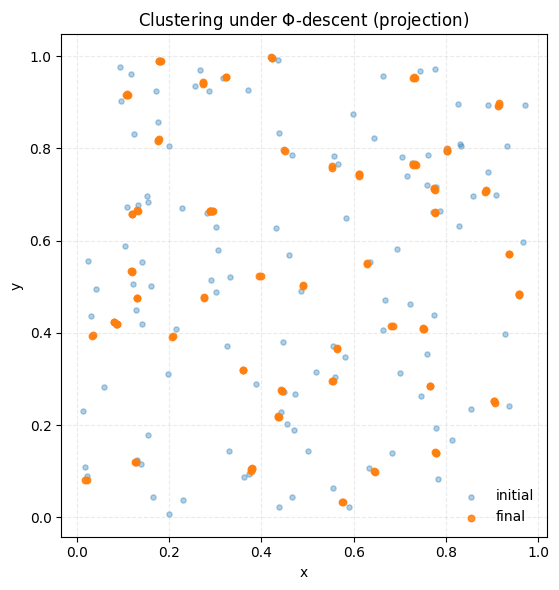
\includegraphics[width=0.82\textwidth]{figures/clustering.png}\caption{\textbf{Clustering under $\Phi$-descent} ($N{=}120$, $\beta{=}10$). Orange: final; blue: initial.}\label{fig:clustering}\end{figure}
\begin{figure}[H]\centering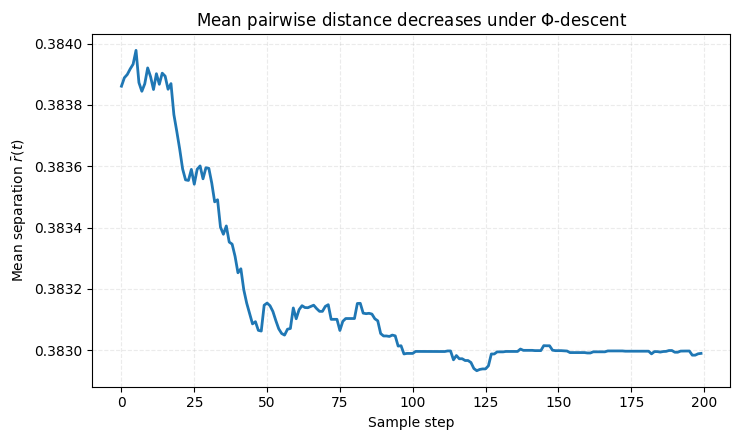
\includegraphics[width=0.75\textwidth]{figures/mean_distance.png}\caption{$\bar r(t)$ decreases under $\Phi$-descent. Error bars: one s.d. over 24 runs; band: IQR.}\label{fig:mean}\end{figure}
\begin{figure}[H]\centering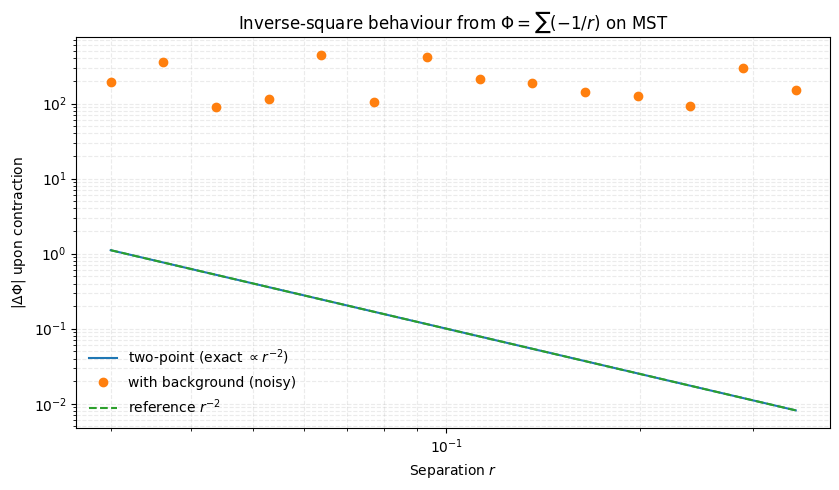
\includegraphics[width=0.9\textwidth]{figures/inverse_square.png}\caption{$\Delta\Phi$ vs $r$ on log--log axes. Reference $r^{-2}$ dashed; analytic two-point curve (solid); many-body points scatter around slope. Error bars: one s.d.; band: IQR.}\label{fig:inverse}\end{figure}
\begin{figure}[H]\centering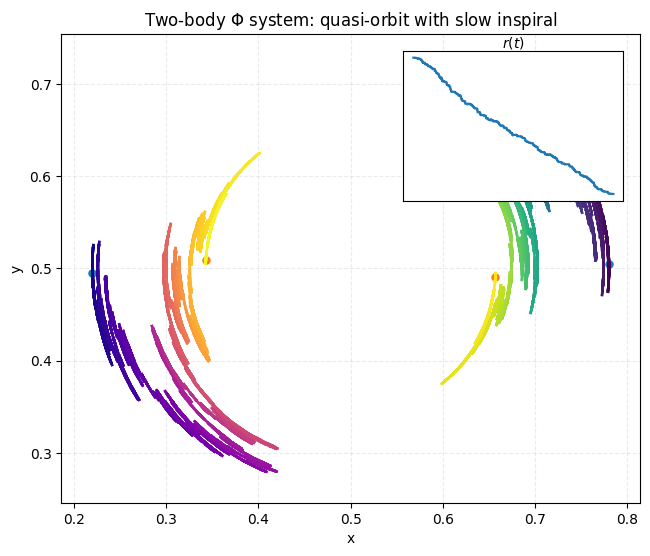
\includegraphics[width=0.78\textwidth]{figures/orbit_two_body.png}\caption{Two-body quasi-orbit with intermittent radial-compression events.}\label{fig:twoorbit}\end{figure}
\begin{figure}[H]\centering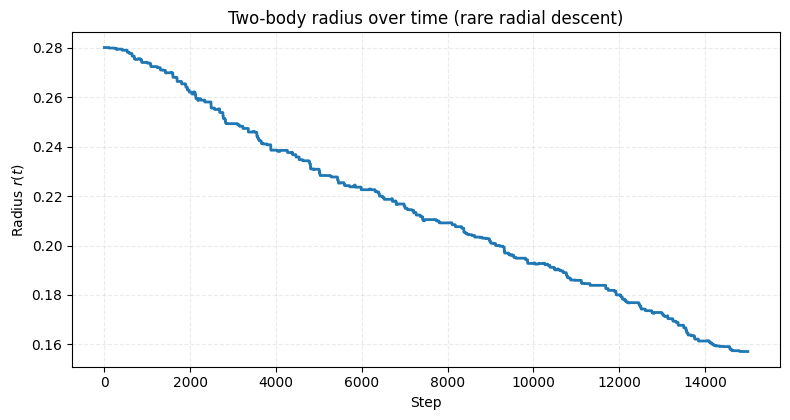
\includegraphics[width=0.88\textwidth]{figures/two_body_r_vs_t.png}\caption{Staircase decrease of $r(t)$ with rare accepted radial steps.}\label{fig:tworadius}\end{figure}
\begin{figure}[H]\centering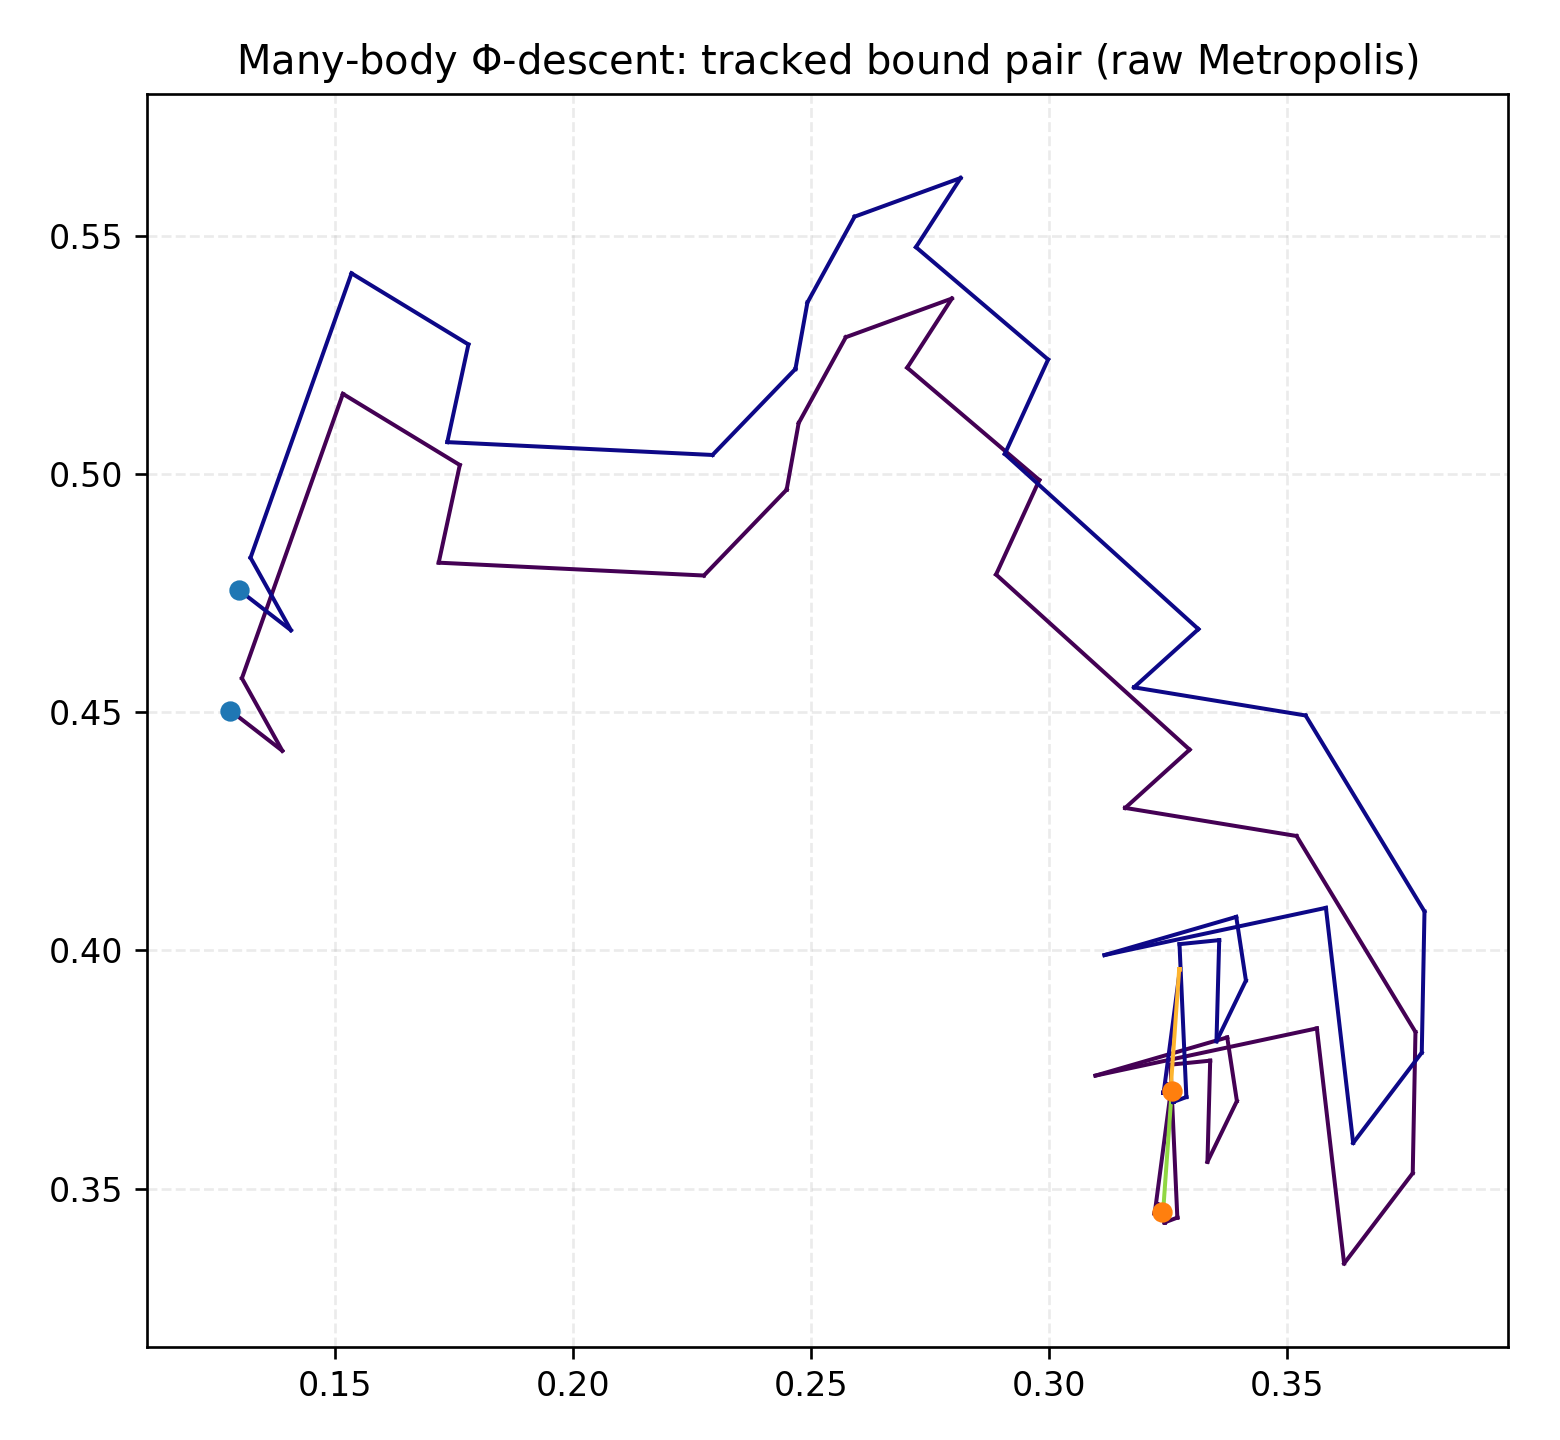
\includegraphics[width=0.86\textwidth]{figures/orbit_many_body.png}\caption{Tracked bound pair in many-body run (start $\bullet$, end $\CIRCLE$).}\label{fig:manypair}\end{figure}

\paragraph*{Code Availability.} Code and figure scripts are available at:\\
\url{https://github.com/Snassy-icp/law_of_minimal_description/tree/main/code/simulations}

% ========================= 11 =========================
\section{Predictions and Falsifiability}
\begin{enumerate}
\item Quantum-scale gravity deviation: $\varepsilon_g(r)\approx\eta(r_0/r)^p$, $\eta\sim10^{-4}$--$10^{-2}$.
\item Entanglement-assisted gravity: $\delta_{\mathrm{ent}}\sim10^{-6}$--$10^{-4}$.
\item No particle dark matter: rotation curves from $\psi_{\text{desc}}(R)\propto\ln R$.
\item Dark energy evolution: $w(z)=-1+\delta w(z)$ with $\delta w\lesssim0.05$.
\item Statistical time symmetry breaking: reversal excess $1+\xi$, $\xi\sim10^{-3}$.
\end{enumerate}

% ========================= 12 =========================
\section{Responses to Common Objections (Rebuttal Appendix)}\label{app:E}
\paragraph*{Uncomputability of $K$.} $K$ is an ideal extremal quantity; physics routinely employs non-computable ideals. Universal MDL surrogates yield gradients consistent with $-\nabla\Phi$ almost everywhere (App.~G).

\paragraph*{Entropy vs. description length.} $\mathbb{E}[K]=H+O(1)$ and $S=k\ln2\cdot H$. Global $\Phi_{\text{tot}}=L(M)+L(D|M)$ decreases while subsystem $S$ may increase; exported entropy pays Landauer cost (Sec.~\ref{sec:sign}).

\paragraph*{Mass and information.} $\rho\propto\rho_m$ is operational via microstate multiplicity and storage energy. Attraction follows from isotropy and flux conservation.

\paragraph*{Geometry from description.} Second variation defines $g_{\mu\nu}$; locality and diffeomorphism invariance select Einstein dynamics via Lovelock.

\paragraph*{Quantum formalism.} Unitary = code-preserving; incompatible codebooks encode non-commutation; entanglement = algorithmic mutual information; MDL selection yields Born rule.

% ========================= 13 =========================
\section{Spatial Dimensionality from Compression and Locality (Heuristic)}\label{app:F}
We seek $n$ admitting: (i) local, isotropic, scale-free kernels with conserved flux; (ii) harmonic Green’s functions with finite-energy bound structures; (iii) additive compression flux. These pick $k'(r)\propto r^{-(n-1)}$. For $n=1,2$ structures are unstable/trivial; for $n\ge4$ scale-free kernels fail to support both finite local flux and stability. In $n=3$, $k(r)=1/r$ is harmonic and supports stable flux. \emph{Heuristic proposition:} under (i)--(iii), $n=3$ minimizes dimension while supporting nontrivial compressive structure.

% ========================= 14 =========================
\section{Gradient Consistency for Universal MDL Estimators (Details)}\label{app:G}
\paragraph*{Setup.} Let $(X,\mathcal{B},\mu)$ be a smooth $\sigma$-finite measure space absolutely continuous with respect to Lebesgue measure in charts. Admissible estimators $\widehat\Phi$ are prefix-free, local, universal (there exists $c$ with $\widehat\Phi\le\Phi+c$), and refinement-stable (code updates supported on finite neighborhoods).

\paragraph*{Theorem (Gradient Consistency).} For any $\widehat\Phi$ admissible and $\mu$-a.e. $x\in X$, there exists a full-measure cone $\mathcal{C}*x$ of directions such that
[
\lim*{h\to0^+}\frac{\widehat\Phi(x+h v)-\widehat\Phi(x)}{h}=\lim_{h\to0^+}\frac{\Phi(x+h v)-\Phi(x)}{h}.
]
\emph{Sketch.} (1) Universality bounds $|\widehat\Phi-\Phi|$. (2) Locality/refinement-stability bound code updates under small displacements. (3) Discontinuities of $K$ lie in a $\mu$-null set; restrict to typical $x$. (4) Symmetric-difference of codebooks vanishes as $h\to0^+$, giving equality almost everywhere. \hfill$\square$

% ========================= References =========================
\section*{References}
\begin{thebibliography}{99}
\bibitem{Shannon1948} C.~E.~Shannon, `A Mathematical Theory of Communication,'' \emph{Bell Syst. Tech. J.} (1948).
\bibitem{CoverThomas} T.~M.~Cover and J.~A.~Thomas, \emph{Elements of Information Theory}, 2nd ed. (Wiley, 2006).
\bibitem{LiVitanyi} M.~Li and P.~Vit\'anyi, \emph{An Introduction to Kolmogorov Complexity and Its Applications}, 3rd ed. (Springer, 2008).
\bibitem{Rissanen1978} J.~Rissanen, `Modeling by Shortest Data Description,'' \emph{Automatica} (1978).
\bibitem{Solomonoff64} R.~J.~Solomonoff, `A Formal Theory of Inductive Inference,'' \emph{Inf. Control} (1964).
\bibitem{Hutter} M.~Hutter, \emph{Universal Artificial Intelligence} (Springer, 2005).
\bibitem{Jaynes1957} E.~T.~Jaynes, `Information Theory and Statistical Mechanics,'' \emph{Phys. Rev.} (1957).
\bibitem{Zurek2003} W.~H.~Zurek, `Decoherence, Einselection, and the Quantum Origins of the Classical,'' \emph{Rev. Mod. Phys.} (2003).
\bibitem{Amari2016} S.-I.~Amari, \emph{Information Geometry and Its Applications} (Springer, 2016).
\bibitem{Landauer1991} R.~Landauer, `Information is Physical,'' \emph{Physics Today} (1991).
\bibitem{Bennett1982} C.~H.~Bennett, `The Thermodynamics of Computation,'' \emph{Int. J. Theor. Phys.} (1982).
\bibitem{Newton1687} I.~Newton, \emph{Philosophi\ae\ Naturalis Principia Mathematica} (1687).
\bibitem{Einstein1916} A.~Einstein, `The Foundation of the General Theory of Relativity,'' \emph{Ann. Phys.} (1916).
\bibitem{MTW1973} C.~W.~Misner, K.~S.~Thorne, J.~A.~Wheeler, \emph{Gravitation} (Freeman, 1973).
\bibitem{Wald1984} R.~M.~Wald, \emph{General Relativity} (Chicago, 1984).
\bibitem{Lovelock1971} D.~Lovelock, `The Einstein Tensor and Its Generalizations,'' \emph{J. Math. Phys.} (1971).
\bibitem{Schmidhuber2000} J.~Schmidhuber, `Algorithmic Theories of Everything,'' arXiv:quant-ph/0011122 (2000).
\bibitem{Lloyd2006} S.~Lloyd, \emph{Programming the Universe} (Knopf, 2006).
\bibitem{Feynman1948} R.~P.~Feynman, `Space-Time Approach to Non-Relativistic Quantum Mechanics,'' \emph{Rev. Mod. Phys.} (1948).
\bibitem{Holland1993} P.~Holland, \emph{The Quantum Theory of Motion} (CUP, 1993).
\bibitem{Jackson1998} J.~D.~Jackson, \emph{Classical Electrodynamics}, 3rd ed. (Wiley, 1998).
\bibitem{Jacobson1995} T.~Jacobson, `Thermodynamics of Spacetime: The Einstein Equation of State,'' \emph{Phys. Rev. Lett.} \textbf{75}, 1260--1263 (1995).
\bibitem{Verlinde2011} E.~Verlinde, `On the Origin of Gravity and the Laws of Newton,'' \emph{JHEP} \textbf{04} (2011) 029.
\bibitem{CatichaED} A.~Caticha, \emph{Entropic Dynamics}, various (2011--2022).
\bibitem{Prim1957} R.~C.~Prim, `Shortest Connection Networks and Some Generalizations,'' \emph{Bell Syst. Tech. J.} \textbf{36}, 1389--1401 (1957).
\end{thebibliography}

\end{document}
